\section{The Early Visual System}
\label{sec:EarlyVisualSystem}
\begin{prin}[Retinal Signal Conversion]
  \label{prin:retina}
  The conversion of a light stimulus into an electrical signal and ultimately an action potential sequence occurs in the retina.
  The retina is roughly composed of 3 layers of cells, \emph{photoreceptor cells}, \emph{bipolar cells} and \emph{ganglion cells}. First, photoreceptor cells convert light signals into electrical signals. And then, bipolar cells are responsible for sorting and processing these electrical signals. Finally, ganglion cells will convert electrical signals into action potential sequences.
   In the intact eye, counterintuitively, light enters through the side opposite from the photoreceptors because Vertebrate retinal cell layers are arranged in reverse order of signaling.
\end{prin}

\begin{rem}
   Changing membrane potentials is adequate for signaling within the retina, where distances are small. However, it is inadequate for the task of conveying information from the retina to the brain. Thus, the ganglion cells are needed.
\end{rem}

\begin{exm}
  The following figure A is an anatomical diagram showing the five principal cell types of the retina and figure B is a rough circuit diagram and intracellular recordings made in neurons of the retina of a mud puppy (an amphibian). The rod cells, especially the one on the left side of figure B, are hyperpolarized by the light flash. This electrical signal is passed along to bipolar and horizontal cells through synaptic connections. Note that in one of the bipolar cells, the signal has been inverted, leading to depolarization. Pluses and minuses represent excitatory and inhibitory synapses, respectively.
  The two retinal ganglion cells shown in the figure have different responses and transmit different sequences of action potentials. $G_2$ fires while the light is on, and $G_1$ fires when it turns off. These are called \emph{ON} and \emph{OFF responses}, respectively
  \begin{center}
    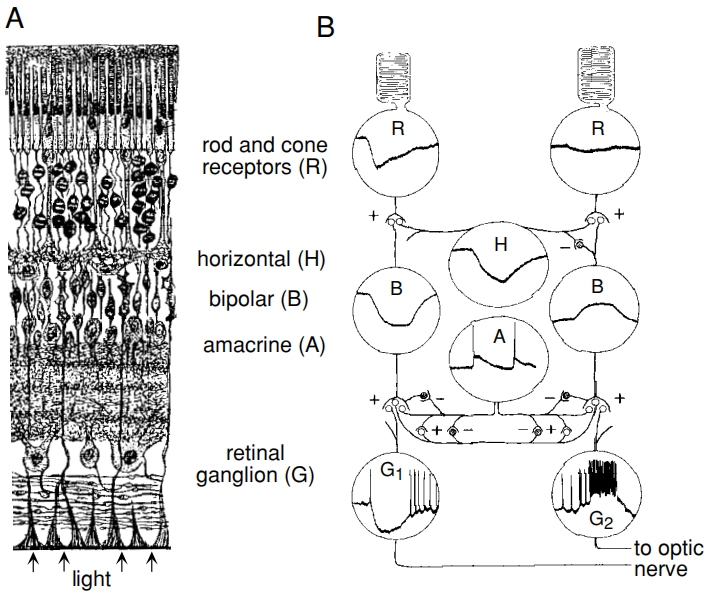
\includegraphics[scale=0.25]{./png/dogRetina}
  \end{center}
\end{exm}

\begin{ntn}
  \label{ntn:opticNerve}
  The output neurons of the retina are the retinal ganglion cells, whose axons form the \emph{optic nerve}.
\end{ntn}

\begin{prin}[Visual Pathway]
  \label{prin:visualPathway}
  As the following figure shows, the optic nerve carry information from each visual hemifield up to the \emph{optic chiasm}, where some retinal ganglion cell axons cross the midline at the optic chiasm, and then to the LGN. Cells in this nucleus send their axons along the optic radiation to the primary visual cortex.
  \begin{center}
    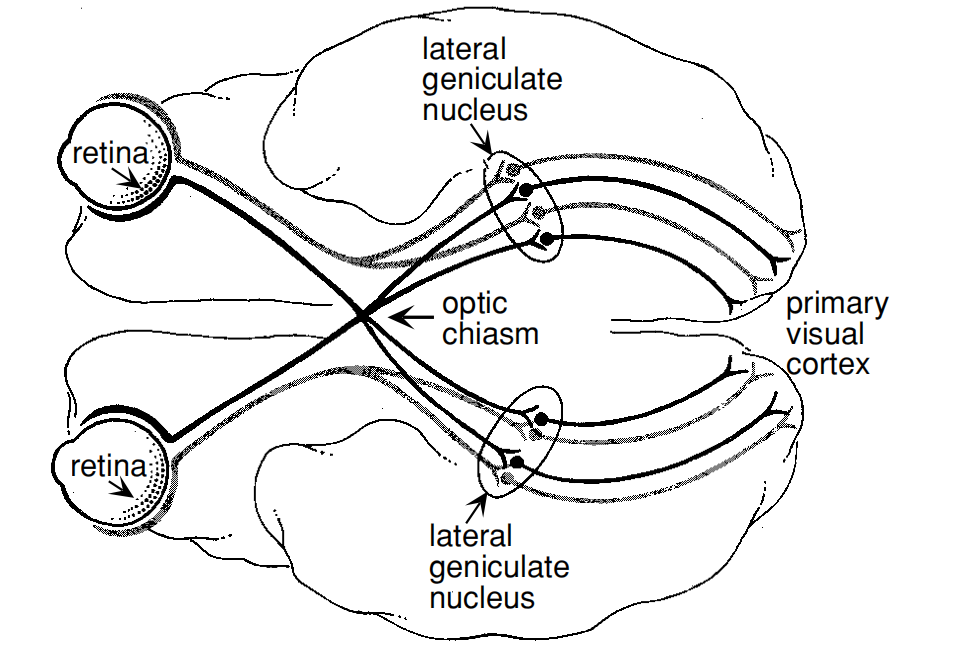
\includegraphics[scale=0.2]{./png/visualPathway}
  \end{center}
\end{prin}

\begin{defn}
  \label{def:visualReceptiveField}
  The restricted regions of the visual field where light stimuli could active Neurons in the retina, LGN, and primary visual cortex is called \emph{receptive fields} of the corresponding visual neuron.
\end{defn}

\begin{asm}
  \label{asm:OutsideRecept}
  Patterns of illumination outside the receptive field of a given neuron cannot generate a response directly, although they can significantly affect responses to stimuli within the receptive field. We do not consider such effects, although they are of considerable experimental and theoretical interest.
\end{asm}

\begin{rem}
  Within the receptive fields, there are regions where illumination higher than the background light intensity enhances firing, and other regions where lower illumination enhances firing. The spatial arrangement of these regions determines the selectivity of the neuron to different inputs. The term \emph{receptive field} is often generalized to refer not only to the overall region where light affects neuronal firing, but also to the spatial and temporal structure within this region.
\end{rem}

\begin{ntn}
  \label{simpleComplexCells}
  Visually responsive neurons in the retina, LGN, and primary visual cortex are divided into two classes, depending on whether or not the contributions from different locations within the visual field sum linearly. \emph{Simple cells} in primary visual cortex appear to satisfy this assumption. \emph{Complex cells} in primary visual cortex do not show linear summation across the spatial receptive field, and nonlinearities must be included in descriptions of their responses.
\end{ntn}

\begin{asm}
  \label{asm:light}
  To streamline the discussion in this chapter, we consider only gray-scale images, although the methods presented can be extended to include color. We also restrict the discussion to two-dimensional visual images, ignoring how visual responses depend on viewing distance and encode depth.
\end{asm}

\begin{rem}
  In discussing the response properties of retinal, LGN, and V1 neurons, we do not follow the path of the visual signal, nor the historical order of experimentation, but instead begin with primary visual cortex and then move back to the LGN and retina. And the emphasis of this chapter is on properties of individual neurons.
\end{rem}

\subsection{The Retinotopic Map}
\label{sec:retinotopicMap}
\begin{defn}
  \label{def:retinotopicMap}
  The \emph{retinotopic map} is a map from the visual world to the cortical surface that make sure neighboring points in a visual image evoke activity in neighboring regions of visual cortex. 
\end{defn}

\begin{rem}
  The retinotopic map refers to the transformation from the coordinates of the visual world to the corresponding locations on the cortical surface.
\end{rem}

\begin{ntn}
  \label{fixationPoint}
  The image point that focuses onto the fovea or center of the retina is called the \emph{fixation point}.
\end{ntn}

\begin{ntn}
  \label{ntn:twoCoordinateSystems}
  Polar and Cartesian coordinate systems used to parameterize image location is shown in the following figure. Each rectangle represents a tangent screen, and the filled circle is the location of a particular image point on the screen.
  \begin{center}
    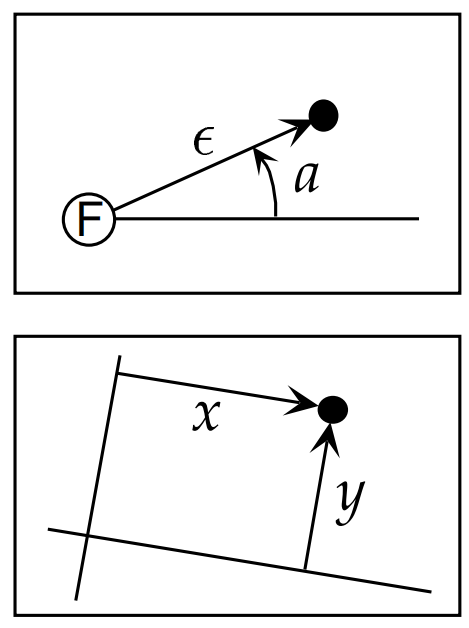
\includegraphics[scale=0.15]{./png/Coord}
  \end{center}
  The origin of the polar coordinate system is the fixation point F, the \emph{eccentricity} $\epsilon$ is proportional to the radial distance from the fixation point to the image point, and \emph{azimuth} $a$ is the angle between the radial line from F to the image point and the horizontal axis. The origin and the orientation of the axes are usual chosen to center and align the coordinate system with respect to a particular receptive field being studied.
\end{ntn}

 
 




%%% Local Variables:
%%% mode: latex
%%% TeX-master: "../notesOnFluidMechanics"
%%% End:
